\chapter{Methodik}
\label{chap:methodik}

In diesem Kapitel wird die Methodik beschrieben, die für die Entwicklung des Frameworks verwendet wird, das ML-Modelle für den Einsatz auf Embedded Systems optimiert. 
Dazu gehören die Durchführung der \textbf{Literaturrecherche}, die \textbf{Anforderungsanalyse} \cite{10433185} sowie die Auswahl der \textbf{Entwicklungsumgebung}, die verwendeten 
\textbf{Optimierungstechniken} \cite{9838829} und die \textbf{Implementierungsschritte} für das Framework. Der Fokus liegt auf der effizienten Ausführung von ML-Modellen auf 
ressourcenbeschränkten Geräten wie SPS und IPC in der industriellen Fertigung.

\section{Literaturrecherche und Anforderungsanalyse}

Um eine fundierte Basis für die Entwicklung des Frameworks zu schaffen, sind sowohl eine strukturierte Literaturrecherche als auch eine Anforderungsanalyse durchgeführt.
\subsection{Literaturrecherche}

Die Literaturrecherche dient dazu, aktuelle Ansätze und Techniken im Bereich der Embedded Systems und des Machine Learning in der Industrie 4.0 zu identifizieren. 
Folgende Schritte sind befolgt:
\begin{quote}
\textbf{Prozess:}
\begin{enumerate}
\item Definition der Forschungsfrage: Die zentrale Fragestellung zielt darauf ab, die Herausforderungen und Lösungsansätze zur effizienten Implementierung von ML-Modellen auf Embedded Systems in industriellen Anwendungen zu identifizieren \cite{9427249}.
\item Festlegung der Suchstrategie: Relevante wissenschaftliche Datenbanken wie IEEE Xplore \cite{9427249}, ACM Digital Library \cite{ACMDigitalLibrary} und SpringerLink \cite{SpringerLink}sind genutzt. Suchbegriffe wie „Embedded Systems“, „Machine Learning“, „Edge Computing“ und „Industrie 4.0“ bilden die Grundlage für die Suche.
\item Filterung und Auswahl: Durch spezifische Inklusions- und Exklusionskriterien, wie Veröffentlichungsjahr und Relevanz für industrielle Anwendungen, sind die Suchergebnisse eingegrenzt. Insgesamt sind über 50 Fachartikel und Berichte analysiert, von denen 30 für die weitere Untersuchung relevant sind.
\item Analyse und Synthese: Die ausgewählten Artikel werden systematisch analysiert und die Ergebnisse in Bezug auf Schlüsselthemen und Herausforderungen zusammengefasst.
\end{enumerate}
\end{quote}
\subsection{Anforderungsanalyse}

Parallel zur Literaturrecherche wird eine Anforderungsanalyse durchgeführt, um spezifische Anforderungen der Industriepartner zu berücksichtigen. Diese Analyse folgt einem strukturierten Ansatz:
\begin{quote}
\textbf{Prozess:}
\begin{enumerate}
\item \textbf{Interviews und Workshops mit Industriepartnern}: Zur Identifikation praxisrelevanter Anforderungen werden Interviews und Workshops mit Industriepartnern durchgeführt, die Embedded Systems im Produktionsumfeld einsetzen. Hier werden Anforderungen bezüglich Rechenleistung, Energieeffizienz, Echtzeitanforderungen und Modellflexibilität identifiziert.
\item \textbf{Analyse der technischen Dokumentationen}: Technische Spezifikationen der verwendeten Hardware (z. B. SPS und IPC) werden untersucht, um Hardware-Einschränkungen und Schnittstellenanforderungen zu berücksichtigen.
\item \textbf{Kategorisierung der Anforderungen}: Die identifizierten Anforderungen werden in technische und funktionale Anforderungen unterteilt. Technische Anforderungen beziehen sich auf die Hardwareeinschränkungen und notwendige Optimierungstechniken, während funktionale Anforderungen Aspekte wie Echtzeitfähigkeit und Robustheit umfassen.
\item \textbf{Priorisierung}: Anforderungen sind priorisiert, um sicherzustellen, dass die wichtigsten Kriterien wie Echtzeitanforderungen und Effizienz bei der Entwicklung des Frameworks berücksichtigt sind.
\end{enumerate}
\end{quote}

\section{Framework-Entwurf}

Der erste Schritt zur Entwicklung des Frameworks ist die Definition der Anforderungen basierend auf den spezifischen Einschränkungen von Embedded Systems. 
Diese Anforderungen sind in Zusammenarbeit mit Industriepartnern und durch eine umfassende Literaturrecherche zu bestehenden Lösungen festgelegt. Hierbei sind nicht 
nur die Optimierung und Konfiguration der ML-Modelle berücksichtigt, sondern auch Aspekte wie die Datenverarbeitung, Priorisierung von Aufgaben, Logging und das Deployment 
von Modellen auf unterschiedlichen Zielplattformen. Die Schwerpunkte des Frameworks liegen auf:
\begin{itemize}
    \item \textbf{Reduzierung der Modellgröße}: Um die effiziente Ausführung von ML-Modellen auf ressourcenbeschränkten Embedded Systems wie SPS oder IPCs zu ermöglichen, 
    wird die Modellgröße reduziert, ohne dass die Genauigkeit signifikant leidet. Dies ist besonders für Echtzeitanwendungen entscheidend.   
    \item \textbf{Datenverarbeitung und Vorverarbeitung}: Neben der Modelloptimierung ist eine effiziente Datenverarbeitung erforderlich. Die Vorverarbeitung von Sensordaten 
    erfolgt in Echtzeit und filtert irrelevante Informationen, um sicherzustellen, dass nur relevante Daten für Modellvorhersagen genutzt sind. Dies unterstützt die Fähigkeit, 
    Entscheidungen in Echtzeit zu treffen.
   
    \item \textbf{Deployment und Aktualisierung der Modelle}: Eine zentrale Herausforderung in industriellen Umgebungen ist das flexible Deployment von ML-Modellen auf 
    verschiedenen Geräten (SPS, IPCs etc.). Das Framework ermöglicht eine einfache Bereitstellung neuer oder aktualisierter Modelle, ohne den Produktionsprozess zu stören, 
    und bietet ein robustes Update-Management für nahtlose Integration in bestehende Systeme.
  
    \item \textbf{Priorisierung von Aufgaben}: In Produktionsumgebungen ist die Priorisierung bestimmter Aufgaben zur Erfüllung von Betriebsanforderungen notwendig. 
    Das Framework bevorzugt daher priorisierte Tasks gegenüber weniger kritischen Aufgaben, was insbesondere bei begrenzten Ressourcen und parallelem Prozessbetrieb entscheidend ist.
   
    \item \textbf{Logging und Überwachung}: Um die Systemausführung und -wartung zu unterstützen, integriert das Framework ein umfassendes Logging- und Überwachungssystem. 
    Dieses protokolliert Modellvorhersagen sowie Systemstatusinformationen (z.B. Ressourcenauslastung, Latenzen) und dient der Identifikation von Fehlern, der 
    Leistungsüberwachung und der langfristigen Wartung des Systems.
  
    \item \textbf{Sicherstellung der Echtzeitfähigkeit}: Da viele industrielle Anwendungen Echtzeitanforderungen erfordern, stellt das Framework sicher, dass 
    Vorhersagen innerhalb vorgegebener Zeitgrenzen getroffen sind. Dies erfordert eine optimierte Laufzeitleistung und die Einhaltung zeitlicher Anforderungen des Produktionsprozesses.
   
    \item \textbf{Einfache Integration in bestehende industrielle Steuerungssysteme}: Das Framework ist so konzipiert, dass es sich problemlos in bestehende Steuerungsarchitekturen 
    (wie IPC oder SPS) integriert, um den Einsatz ohne grundlegende Änderungen an der Infrastruktur zu ermöglichen.
\end{itemize}

Das Framework wird als Middleware entwickelt, die als Adapter zwischen den ML-Modellen und den Zielsystemen (SPS, IPC) fungiert. Es unterstützt verschiedene Optimierungstechniken, 
um die Ausführung der Modelle auf hardwarebeschränkten Systemen zu ermöglichen.

\section{Programmiersprachen und Entwicklungsumgebungen}

\subsection{Python}
Python ist eine der am häufigsten verwendeten Programmiersprachen für Machine Learning \cite{info11040193} und bietet eine Vielzahl von Bibliotheken und Frameworks, 
die für industrielle Anwendungen und Embedded-Modelle nützlich sind. Es ist bekannt für seine \textbf{einfache Handhabung} und große Community, 
was es zur ersten Wahl für viele ML-Entwickler macht.

\begin{itemize}
    \item \textbf{TensorFlow und TensorFlow Lite}: TensorFlow bietet eine leistungsstarke Umgebung für die Entwicklung von neuronalen Netzen \cite{8110869}. 
    TensorFlow Lite wurde speziell entwickelt, um TensorFlow-Modelle für ressourcenbeschränkte Geräte zu optimieren und diese auf Embedded-Systemen lauffähig zu machen\cite{9919465}.
    
    \item \textbf{scikit-learn}: Dieses Framework bietet eine umfassende Bibliothek für klassische Machine-Learning-Algorithmen wie 
    Entscheidungsbäume, Random Forests, Support Vector Machines (SVMs), lineare Modelle, K-Means und mehr. Diese Modelle sind oft weniger rechenintensiv 
    und daher für viele industrielle Anwendungen gut geeignet \cite{10306026}.

    \item \textbf{XGBoost}: XGBoost ist bekannt für seine Effizienz und Leistung bei Gradient-Boosting-Modellen und eignet sich gut für industrielle Anwendungen 
    wie Anomalieerkennung, Qualitätskontrolle und vorausschauende Wartung\cite{10603118}.

    \item \textbf{LightGBM}: LightGBM bietet eine ähnliche Funktionalität wie XGBoost, ist jedoch für größere Datensätze und schnellere Trainingszeiten optimiert. 
    Es wird häufig in Echtzeitanwendungen verwendet \cite{9123302}.

    \item \textbf{PyTorch}: PyTorch ist eine flexible Alternative zu TensorFlow, insbesondere für Forschungsprojekte und Produktionssysteme, 
    die dynamische Berechnungsgrafen erfordern. Es wird auch in Embedded-ML-Anwendungen verwendet, wenn größere Modelle benötigt sind\cite{9776868}.

    \item \textbf{CatBoost}: Ein Gradient-Boosting-Framework, das speziell für den Umgang mit kategorischen Daten entwickelt wurde. 
    CatBoost eignet sich besonders gut für industrielle Anwendungen, bei denen viele der Eingabedaten kategorisch sind\cite{10303419}.

    \item \textbf{ONNX}: ONNX bietet eine plattformübergreifende Möglichkeit, ML-Modelle zu konvertieren und auszuführen, die in verschiedenen Frameworks wie 
    TensorFlow, PyTorch oder scikit-learn entwickelt wurden. ONNX erleichtert das Deployment von Modellen auf Embedded- und Edge-Geräten \cite{9730351}.
\end{itemize}

\subsection{Rust}
Rust ist eine moderne Systemprogrammiersprache, die besonders für ihre Speicher- und Speichersicherheitsfunktionen bekannt ist. 
Sie wird zunehmend für Embedded- und Edge-Anwendungen verwendet, da sie hohe Leistung und Sicherheit bietet\cite{arewelearningyet}.

\begin{itemize}
    \item \textbf{Rust-ML-Bibliotheken}: Obwohl Rust weniger bekannt für Machine Learning ist als Python, gibt es Bibliotheken wie \textbf{Linfa}, 
    die klassische ML-Algorithmen wie lineare Regression, K-Means und Entscheidungsbäume bieten.

    \item \textbf{Tch-RS (PyTorch in Rust)}: Tch-RS ist eine Rust-Bindung für PyTorch, die es ermöglicht, PyTorch-Modelle in der Rust-Umgebung zu verwenden. 
    Diese Bibliothek bietet Zugriff auf viele der in PyTorch vorhandenen Funktionen und kann in eingebetteten Umgebungen verwendet sind, in denen Rust bevorzugt wird.

    \item \textbf{SmartCore}: Eine weitere Machine-Learning-Bibliothek in Rust, die viele der klassischen ML-Algorithmen wie Entscheidungsbäume, 
    Random Forests und lineare Modelle unterstützt. Sie eignet sich gut für eingebettete Anwendungen, bei denen Performance und Sicherheit eine Rolle spielen.

    \item \textbf{ONNX mit Rust}: ONNX kann auch in Rust integriert sind, um neuronale Netze oder klassische Modelle, die in anderen Frameworks entwickelt wurden, 
    auf Embedded-Systemen bereitzustellen.
\end{itemize}

Diese Programmiersprachen und Tools bieten wertvolle Möglichkeiten für industrielle Anwendungen im Bereich der künstlichen Intelligenz und Embedded-Systeme, 
mit Schwerpunkten auf Effizienz, Flexibilität und Ressourcenschonung.

\section{Tools für Modelloptimierung, Konvertierung und Deployment}

Zur Optimierung, Konvertierung und Bereitstellung von ML-Modellen auf Embedded Systems stehen verschiedene spezialisierte Tools zur Verfügung. 
Diese Werkzeuge unterstützen die effiziente Ausführung auf ressourcenbeschränkten Geräten und bieten flexible Optionen für die Integration in Produktionsumgebungen.

\textbf{TensorFlow Lite} dient als leichtgewichtige Version von TensorFlow, entwickelt für den Einsatz auf mobilen und eingebetteten Geräten. 
Mit Techniken wie Quantisierung und Pruning reduziert es Modellgröße und Rechenaufwand, was den Einsatz in Echtzeit- und Embedded-Anwendungen ermöglicht.

\textbf{ONNX Runtime} erlaubt die plattformübergreifende Ausführung von ML-Modellen, die in Frameworks wie TensorFlow, PyTorch oder scikit-learn entwickelt wurden. 
Es optimiert Modelle für eine Vielzahl von Hardwareplattformen und ermöglicht ein effizientes Deployment auf Edge- und Embedded-Systemen.

\begin{figure}[h!]
    \centering
    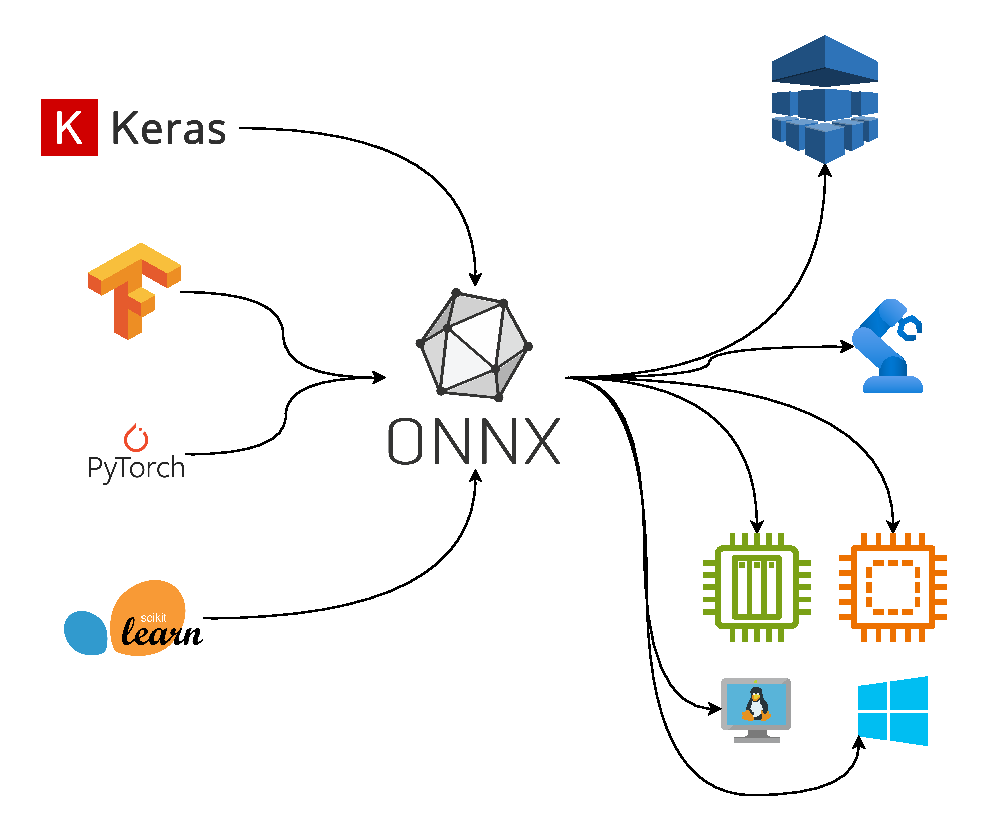
\includegraphics[width=0.9\textwidth]{ONNX.drawio.pdf} 
    \caption{ONNX Runtime für plattformübergreifende ML-Modelle} 
    \label{fig:onnxruntime} % Reference label
\end{figure}

\textbf{Apache TVM} ist ein Compiler-Framework, das ML-Modelle für diverse Hardwarearchitekturen optimiert und speziell an die Anforderungen von Embedded-Geräten anpasst. 
Es unterstützt die effiziente Ausführung auf Mikrocontrollern, GPUs und Edge-Computing-Plattformen.

\textbf{TinyML-Frameworks} wie TensorFlow Micro und uTensor sind darauf ausgelegt, ML-Modelle auf extrem ressourcenbeschränkten Geräten wie Mikrocontrollern auszuführen. 
Diese Frameworks ermöglichen die Implementierung auf Kleinstgeräten ohne Überlastung der Rechenressourcen.

\textbf{TensorRT} von NVIDIA ist ein High-Performance-Optimizer für neuronale Netze und steigert die Inferenzleistung auf NVIDIA-Plattformen wie dem Jetson Nano. 
TensorRT eignet sich besonders für Echtzeitanwendungen auf leistungsstarker Edge-Hardware.

\textbf{Docker} und \textbf{K3s} vereinfachen das Deployment von Modellen durch Containerisierung und Orchestrierung auf Edge- und IoT-Geräten. Docker verpackt Modelle und Abhängigkeiten in Containern für ein konsistentes Deployment, während K3s als leichtgewichtige Kubernetes-Distribution die Verwaltung von ML-Diensten in Edge-Computing-Umgebungen unterstützt.

\textbf{MLflow} bietet eine umfassende Verwaltung des gesamten ML-Modelllebenszyklus. Es unterstützt das Tracking, die Versionierung und das Deployment, was für die Überwachung und Pflege mehrerer Modellversionen in produktiven Systemen vorteilhaft ist.

\textbf{PyInstaller} konvertiert Python-Anwendungen und ML-Modelle in ausführbare Dateien und ermöglicht deren Ausführung auf Geräten ohne Python-Laufzeitumgebung, was das Deployment als eigenständige Anwendung oder Windows-Dienst unterstützt.

\textbf{Zephyr RTOS} stellt ein Echtzeitbetriebssystem bereit, das für die Ausführung von ML-Modellen auf Mikrocontrollern optimiert ist und die Echtzeitanforderungen der industriellen Fertigung erfüllt.

Zusammen bieten \textbf{Conda} und \textbf{Pip} eine umfassende Verwaltung der Modellabhängigkeiten. Conda eignet sich für umfangreiche Bibliotheken wie TensorFlow und PyTorch, da es eine effizientere Verwaltung und Integration großer Bibliotheken ermöglicht. Pip wird für spezialisierte Bibliotheken verwendet, die nicht über Conda verfügbar sind, und ergänzt die Abhängigkeitsverwaltung flexibel.

Diese Tools und Techniken tragen dazu bei, ein Framework zu entwickeln, das ML-Modelle auf Embedded Systems effizient implementiert und die Anforderungen moderner industrieller Anwendungen erfüllt.

\section{Optimierungstechniken}

Die Optimierung von ML-Modellen für Embedded Systems stellt einen wesentlichen Aspekt dieses Projekts dar. Im Folgenden sind die implementierten Techniken beschrieben:

\textbf{Quantisierung} reduziert die Größe eines ML-Modells, indem die Genauigkeit der Gewichtungen von 32-Bit-Gleitkommazahlen auf 8-Bit-Ganzzahlen verringert wird \cite{9919465}. 
Dies führt zu einer erheblichen Senkung des Speicherbedarfs und ermöglicht die Ausführung der Modelle auf Geräten mit begrenzten Ressourcen. Diese Technik wird insbesondere bei 
Modellen eingesetzt, die auf speicher- und rechenkapazitätsbeschränkten Systemen wie SPS und IPCs verwendet sind.


Beim \textbf{Model Pruning} sind nicht benötigte Neuronen und Verbindungen aus dem ML-Modell entfernt, um dessen Größe zu reduzieren, ohne die Genauigkeit signifikant zu beeinträchtigen. 
Diese Technik verbessert die Ausführungsgeschwindigkeit auf Embedded Systems, während die Reduktion der Modellgenauigkeit minimal bleibt \cite{10.1145/3664647.3681449}.

Neben den oben genannten Techniken kommen speziell für Embedded Systems optimierte Algorithmen zur Anwendung. Diese Algorithmen sind auf minimalen Rechenaufwand ausgelegt 
und ermöglichen gleichzeitig Echtzeitentscheidungen. Ein Beispiel hierfür sind \textbf{binäre Entscheidungsbäume} und lineare Modelle, die weniger komplex als neuronale Netzwerke sind, 
jedoch in vielen industriellen Anwendungen eine ausreichende Leistungsfähigkeit bieten.

\section{Implementierungsschritte}

\subsection{Anforderungsanalyse}
Zunächst erfolgt die Erfassung der Anforderungen der industriellen Partner und die Durchführung einer Anforderungsanalyse. Die zentralen Anforderungen fokussieren sich 
auf die Reduktion der Modellgröße, die Sicherstellung der Echtzeitfähigkeit sowie eine ressourcenschonende Ausführung auf Embedded-Devices. Besonders berücksichtigt sind die 
spezifischen Hardware-Einschränkungen der eingesetzten SPS- und IPC-Systeme. Zusätzlich sind Zielfunktionen und Prioritäten festgelegt, um eine Balance zwischen \textbf{Modellkomplexität}, 
\textbf{Laufzeitleistung} und \textbf{Speicherverbrauch} zu erreichen.


\begin{figure}[h!]
    \centering
    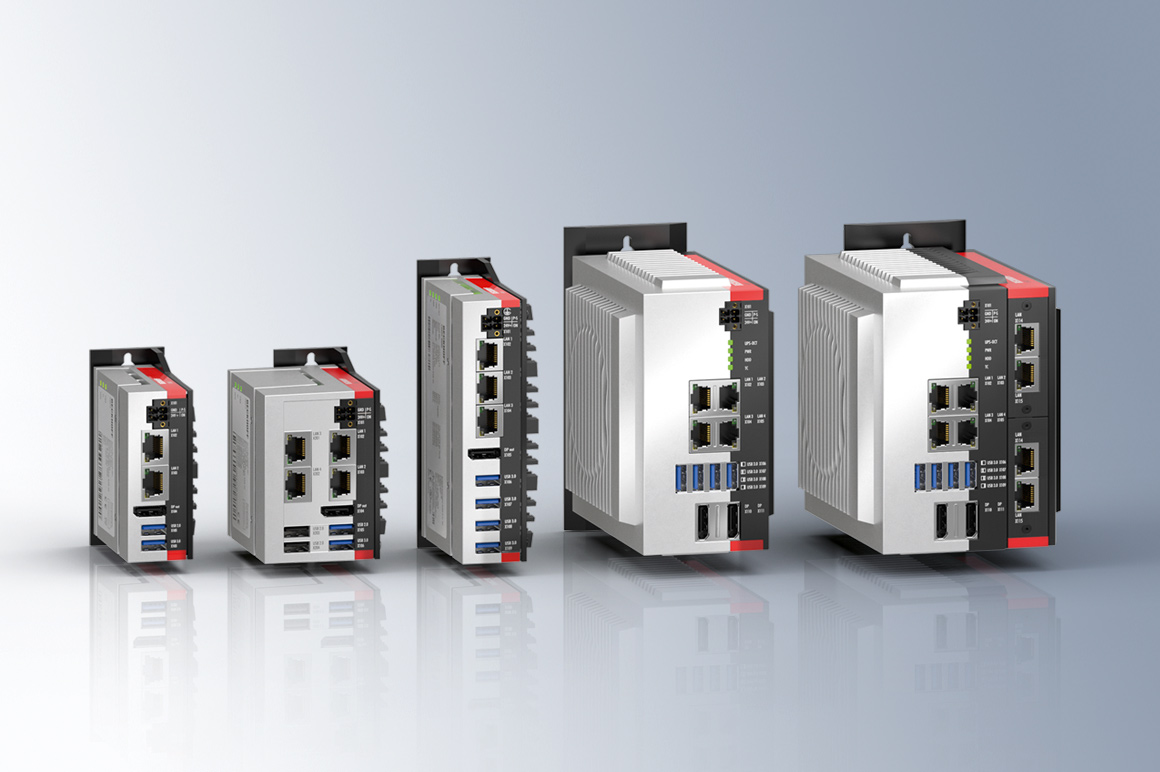
\includegraphics[width=0.6\textwidth]{c60xx-ultra-kompakt-industrie-pcs.jpg} 
    \caption{Beckoff IPCs - C60xx | Ultra-compact Industrial PCs\cite{BeckhoffWebsite}} 
    \label{fig:beckoffipc} % Reference label
\end{figure}


\subsection{Entwicklung des Frameworks}
Das Framework wird als flexible Schnittstelle zwischen den optimierten ML-Modellen und den Embedded Systems entworfen. Die Architektur gliedert sich in verschiedene Module, 
die sowohl die Modelloptimierung als auch die Kommunikation zwischen den Geräten unterstützen. Die wesentlichen Entwicklungsaspekte umfassen:

\begin{itemize}
    \item \textbf{Architekturentwurf}: Die Architektur ist modular aufgebaut, um die Integration und den Austausch verschiedener ML-Modelle zu erleichtern.
    
    \begin{figure}[h!]
        \centering
        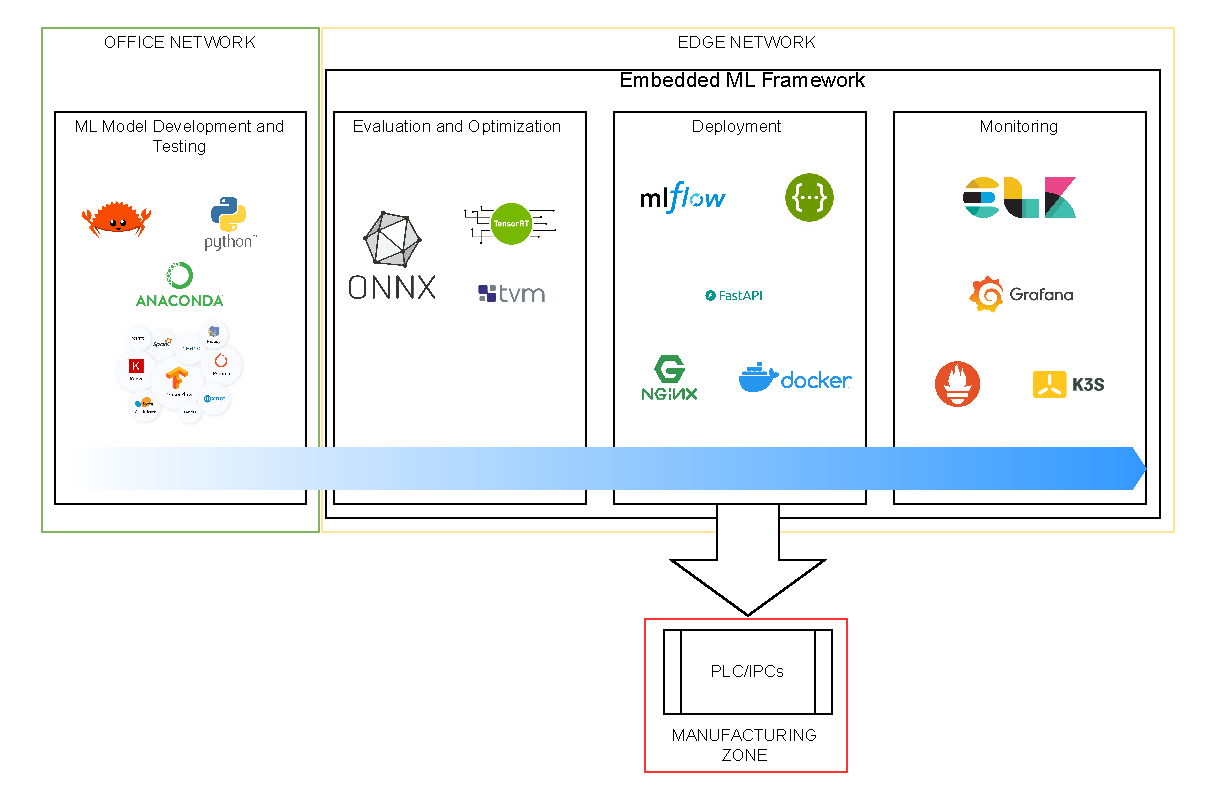
\includegraphics[width=1\textwidth]{Architecture.drawio.pdf} 
        \caption{Architektur des Frameworks} 
        \label{fig:architecture}
    \end{figure}

    \item \textbf{Modelloptimierungstechniken}: Techniken wie Quantisierung, Pruning und Kompression sind eingesetzt, um die Modellgröße zu verringern und die 
    Ausführungseffizienz zu steigern.
    \item \textbf{API-Design}: Eine flexible API ermöglicht den Zugriff auf verschiedene ML-Modelle und gewährleistet eine unkomplizierte Bereitstellung auf unterschiedlichen 
    Embedded Devices.
\end{itemize}

\subsection{Integration und Tests}
Das Framework wird auf verschiedenen Embedded Devices, einschließlich SPS und IPCs, integriert und umfassend getestet. Dieser Schritt beinhaltet:

\begin{itemize}
    \item \textbf{Hardware-Integration}: Die Anpassung des Frameworks an spezifische Hardware-Eigenschaften unterschiedlicher Embedded-Plattformen.
    \item \textbf{Unit-Tests}: Unit-Tests sichern die korrekte Funktionalität der zentralen Komponenten ab.
    \item \textbf{Hardware-in-the-Loop (HIL) Tests}: HIL-Tests \cite{10407700, 10384901} überprüfen das Framework unter realen Bedingungen und stellen sicher, dass die Modelle in Echtzeit mit der Hardware 
    interagieren.
    \item \textbf{Laufzeitleistungsprüfung}: Benchmarks zur Messung der Ausführungszeiten sind definiert, um die Erfüllung der Echtzeitanforderungen industrieller Anwendungen 
    zu gewährleisten.
\end{itemize}

\subsection{Evaluation der Ergebnisse}

Nach der Integration wird das Framework anhand vordefinierter Leistungsmetriken evaluiert:

\begin{itemize}
    \item \textbf{Leistungsmetriken}: Die wichtigsten Metriken umfassen die Ausführungszeit, den Speicherverbrauch und den Energieverbrauch auf den Embedded Devices.
    \item \textbf{Vergleich mit den Anforderungen}: Die Ergebnisse vergleichen mit den in der Anforderungsanalyse definierten Zielwerten, um die Erfüllung der Anforderungen 
    zu validieren.
    \item \textbf{Robustheit und Fehlerbehandlung}: Tests bewerten die Robustheit des Frameworks und dessen Fähigkeit zur Fehlerbewältigung, beispielsweise bei Hardwareausfällen oder 
    Modellfehlern.
    \item \textbf{Optimierungspotential}: Basierend auf den Evaluierungsergebnissen wird weiteres Optimierungspotenzial, wie die Reduktion des Energieverbrauchs oder die Verbesserung 
    der Ausführungszeiten, identifiziert.
\end{itemize}

\begin{table}[h!]
    \caption{Beispiel evaluationsergebnisse des Frameworks}
    \begin{tabular}{|l|c|c|c|c|}
    \hline
    \textbf{Metrik}               & \textbf{Gemessener Wert} & \textbf{Zielwert} & \textbf{Erfüllungsgrad} & \textbf{Opt.Potential} \\ \hline
    Ausführungszeit               & 120 ms                  & $\leq$ 150 ms     & Erfüllt                 & Gering \\ \hline
    Speicherverbrauch             & 512 MB                  & $\leq$ 500 MB     & Teilerfüllt             & Mittel \\ \hline
    Energieverbrauch              & 2.5 W                   & $\leq$ 2 W        & Nicht erfüllt           & Hoch \\ \hline
    Robustheit                    & 95\% Fehlerfrei         & $\geq$ 99\%       & Teilerfüllt             & Hoch \\ \hline
    Fehlerbehandlungskapazität    & 100\% Erfolgreich       & 100\%             & Erfüllt                 & Gering \\ \hline
    \end{tabular}
    \label{tab:evaluation}
\end{table}

\subsection{Zusätzliche Anforderungen}

Weitere Themen die zu beachten sind:

\begin{itemize}
    \item \textbf{Sicherheit und Datenschutz}: Das Framework erfüllt die Datensicherheitsanforderungen der industriellen Fertigung und stellt sicher, dass sensible 
    Informationen geschützt und gemäß den branchenspezifischen Richtlinien verarbeitet sind.
    
    \item \textbf{Flexibilität und Erweiterbarkeit}: Das Framework ist modular und flexibel gestaltet, sodass zukünftige Erweiterungen und die Integration neuer ML-Modelle 
    ohne umfassende Anpassungen möglich sind. Diese Struktur ermöglicht eine hohe Anpassungsfähigkeit an wechselnde industrielle Anforderungen.
    
    \item \textbf{Wartung und Updates}: Implementierte Mechanismen zur Wartung und für Modell-Updates gewährleisten die langfristige Nutzbarkeit und Anpassungsfähigkeit des Frameworks. 
    Durch ein robustes Update-Management können Aktualisierungen und Fehlerbehebungen effizient durchgeführt sind, was die Zuverlässigkeit des Systems steigert.
\end{itemize}

\captionsetup{justification=centering, font=small, labelfont=bf, labelsep=colon}

\definecolor{lightgray}{gray}{0.9}    % Hintergrundfarbe für Header
\definecolor{darkgray}{gray}{0.8}     % Alternierende Hintergrundfarbe für Reihen

\begin{longtable}{|>{\raggedright\arraybackslash}p{4.5cm}|>{\raggedright\arraybackslash}p{10cm}|}
    \caption{Andere Systemvoraussetzungen} \\
    \hline
    \rowcolor{lightgray}
    \textbf{Systemvoraussetzungen} & \textbf{Erläuterung} \\
    \hline
    Cloud Computing & Bereitstellung der leistungsfähigen IT-Infrastruktur für aufwendige Berechnungen, Datenspeicherung und Ausführung über das Internet bezogener Softwareanwendungen. \\
    \hline
    \rowcolor{darkgray}
    Sensorik & Technologien zur Wahrnehmung, Messung und Kontrolle von Veränderungen in der Umgebung oder in einem technischen System. \\
    \hline
    Edge Computing & IT-Infrastrukturen, die eine dezentralisierte Datenspeicherung und -verarbeitung realisieren. \\
    \hline
    \rowcolor{darkgray}
    Datenhoheit, -zugang & Rechtliche Regulierungen, die die Nutzung, Zugang und Verwertung von Daten bestimmen. \\
    \hline
    Datenqualität & Vollständigkeit der Daten, einheitliche Formatierung oder Detaillierungsgrad, unterbrechungsfreie Datenaufnahmen. \\
    \hline
    \rowcolor{darkgray}
    Robustheit der Algorithmen (Reaktion auf unerwartete Situationen) & Zuverlässigkeit der Ergebnisse der Datenanalyse, Reaktion auf Ausreißer und unerwartete Situationen. \\
    \hline
    Trainingsdauer und Aufwand für Algorithmen & Zeit- und Personalaufwand für eine zuverlässige Erkennung von Objekten oder Handlungen, die durch das Sammeln und Annotieren von Trainingsdaten entsteht. \\
    \hline
    \rowcolor{darkgray}
    Rechenaufwand/Energieeffizienz & Aufwendige Berechnungen der Bewegungsabläufe während Aktionsplanung, Prozess- oder Parameteroptimierung unter Berücksichtigung von mehreren Optimierungskriterien. \\
    \hline
    IT-Sicherheit (Security) & Schutz von sensiblen Unternehmensdaten vor Cyberangriffen. \\
    \hline
    \rowcolor{darkgray}
    Funktionale Sicherheit (Safety) & Zuverlässiger und sicherer Betrieb von industriellen Systemen, Minimierung von Verletzungsrisiken und Personenschäden. \\
    \hline
    Interoperabilität der KI-Verfahren und Daten & Übertragbarkeit der KI-Verfahren auf andere Datenquellen, Einheitlichkeit der Datenmodelle und Formate für die Wiederverwendung der Daten und Algorithmen. \\
    \hline
\end{longtable}

\section{Zusammenfassung}
Das Framework basiert auf einer umfassenden Anforderungsanalyse, ist modular und für den Betrieb auf Embedded Devices optimiert. Die effiziente Ausführung 
auf ressourcenbeschränkten Systemen wird durch den Einsatz spezifischer Optimierungstechniken, wie Quantisierung und Pruning, unterstützt. Um die Leistungsfähigkeit des Frameworks 
zu überprüfen, sind detaillierte Tests durchgeführt, die bestätigen, dass Echtzeitfähigkeit und Robustheit den festgelegten Anforderungen entsprechen.

Nach Evaluierung des Frameworks sind zusätzliche Optimierungsmöglichkeiten identifiziert. Diese Verbesserungsbereiche bilden die Grundlage für zukünftige Weiterentwicklungen. 
Zusammenfassend ermöglicht das Framework eine sichere, flexible und performante Implementierung von ML-Modellen auf industriellen Embedded Devices, wobei die Anpassungsfähigkeit an 
neue Anforderungen und eine einfache Wartung gewährleistet sind.